\section{Hardware dell'adapter board}
L'hardware utilizzato per condurre lo studio oggetto di questa tesi consiste in due piattaforme indossabili per effettuare misure fotopletismografiche. Ciascuna piattaforma si compone di una \textit{Adapter Board} e una scheda ospitante un microcontrollore. L'Adapter Board consiste in una PCB sulla quale sono montati il modulo PPG, un accelerometro ed, eventualmente, un regolatore di tensione lineare(LDO) per l'alimentazione dei componenti. Il microcontrollore viene utilizzato per l'acquisizione dei dati dal sensore e per il suo controllo. In particolare, è stata utilizzata in entrambe le soluzioni la board \textbf{STM32F4DISCOVERY}, prodotta da STMicroelectronics, ospitante il microntrollore \textbf{STM32F407}. Grazie poi ad un'interfaccia USB è possibile trasmettere i dati ad un computer per permetterne l'elaborazione e la memorizzazione.
Le due piattaforme si differenziano per l'Adapter Board, in cui sono stati utilizzati due differenti moduli PPG: il \textbf{MAXM86161} e \textbf{MAX86916}, prodotti entrambi da Maxim Integrated.
\subsection{Adapter Board: MAXM86161}
\begin{figure}[b]
	\centering
	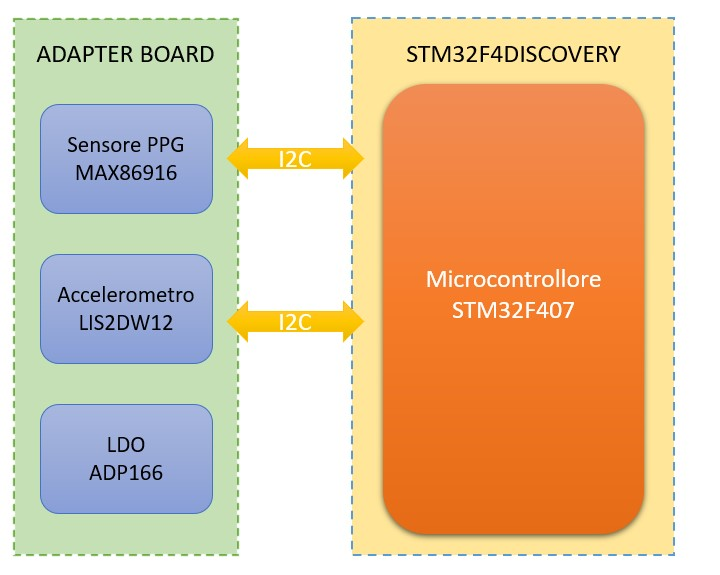
\includegraphics[width=0.6\linewidth]{ImageFiles/Hardware/DiagrammaBlocchiMAXM86161}
	\caption{Diagramma a bloccchi dell'Adapter Board con modulo PPG MAXM86161}
	\label{fig:DiagrammaBlocchiMAXM86161}
\end{figure}
L'Adapter Board progettata ospita il sensore PPG MAXM96161 e l'accelerometro triassiale LIS2DW12, che comunicano con il microcontrollore tramite protocollo I\ap{2}C (\Fig~\ref{fig:DiagrammaBlocchiMAXM86161}). Grazie al numero ridotto di componenti è stato possibile ottenere una scheda dalle dimensioni molto ridotte (12,4 mm x 4,6 mm), con una superficie di appena \SI{57.04}{\square\milli\meter}.

\paragraph{Sensore PPG} Il sensore PPG utilizzato è il MAXM86161 rappresentato nella figura \ref{fig:ImmagineMAXM86161}.
\begin{figure}[tb]
	\centering
	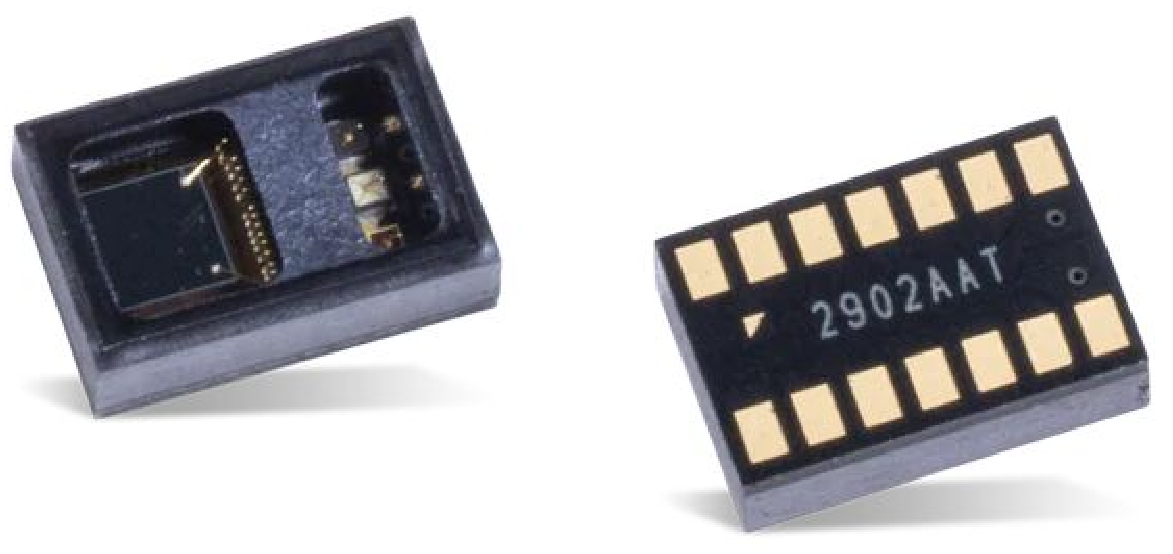
\includegraphics[width=0.7\linewidth]{ImageFiles/Hardware/ImmagineMAXM86161}
	\caption{Il sensore MAXM86161.}
	\label{fig:ImmagineMAXM86161}
\end{figure}
Si tratta di un modulo integrato a basso consumo, per acquisizioni di dati ottici. Il sensore integra 3 LED (rosso, infrarosse e verde), un fotodiodo ed elementi ottici. All'interno è anche presente un regolatore di tensione lineare (LDO). Per questo motivo non è necessario inserire un ulteriore LDO esterno per l'alimentazione dei circuiti interni e dei LED. Il modulo viene alimentato a singola tensione, che deve essere compresa tra i 3.0V e 5.5V. \`E presente un pin di uscita (VLDO) collegato all'uscita del regolatore interno che fornisce una tensione di 1.8V che può essere utilizzato per alimentare eventuali dispositivi esterni. Infatti, nell'Adapter Board, questa uscita è stata utilizzata per alimentare l'accelerometro. 
La comunicazione con il microcontrollore avviene tramite i pin SDA e SCL, tipici della comunicazione I\ap{2}C. Il modulo presenta un package di tipo OLGA a 14 pin, dalle dimensioni ridotte, 2.9 mm x 4.3 mm x 1.4 mm, e un consumo minore di \SI{30}{\micro\watt}.

\paragraph{Accelerometro} Il LIS2DW12 è un accelerometro triassiale lineare, prodotto da STMicroelectronics\cite{STElectronicsLIS2DW12}, realizzato con tecnologia MEMS ad alte performance e basso consumo. 
\begin{figure}[b]
	\centering
	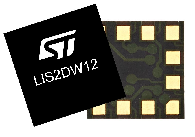
\includegraphics[width=0.3\linewidth]{ImageFiles/Hardware/ImmagineLIS2DW12}
	\caption{Accelerometro LIS2DW12.}
	\label{fig:ImmagineLIS2DW12}
\end{figure}
\`E pensato per rilevazioni di movimento e riconoscimento dei gesti su dispositivi indossabili. Il sensore permette di selezionare un fondo scala di $\pm$\SI{2}{\gram}, $\pm$\SI{4}{\gram}, $\pm$\SI{8}{\gram} oppure $\pm$\SI{16}{\gram}. Necessita di un'alimentazione compresa tra i 1.62V e i 3.6V e la corrente assorbita tipicamente è di \SI{50}{\nano\ampere} nella modalità \textit{power-down} e di \SI{1}{\micro\ampere} in quella attiva \textit{low-power}. Inoltre, l'accelerometro include un sensore di temperatura che permette di compensare gli effetti termici sulle misure. Presenta un'interfaccia I\ap{2}C e un interfaccia SPI per la comunicazione. Questo sensore è stato inserito nell'Adapter Board per ottenre una stima di eventuali disturbi, dovuti agli artefatti del movimento, permettendo quindi di ottenere delle stime dei parametri di qualità superiore. Il sensore è realizzato in un package di tipo LGA-12 con dimensioni 2.0 mm x 2.0 mm x 0.7 mm.

\paragraph{Progetto PCB} Il progetto della board è stato realizzato con il software Autodesk Eagle. Come prima fase del progetto è stato realizzato lo schematico, dove sono state definite le interconnessioni dei componente a livello logico. In seguito, è stato definito il layout della PCB, definendo la posizione dei componenti e delle piste che li connettono.
In figura \ref{fig:schematic_maxm} viene riportato lo schematico dove si possono vedere il sensore PPG, l'accelerometro e due connettori necessari, uno per l'alimentazione della scheda (VCC e GND), e uno per la comunicazione I\ap{2}C e l'interrupt del modulo PPG (SDA, SCL, INT\_PPG).
\begin{figure}[b]
	\centering
	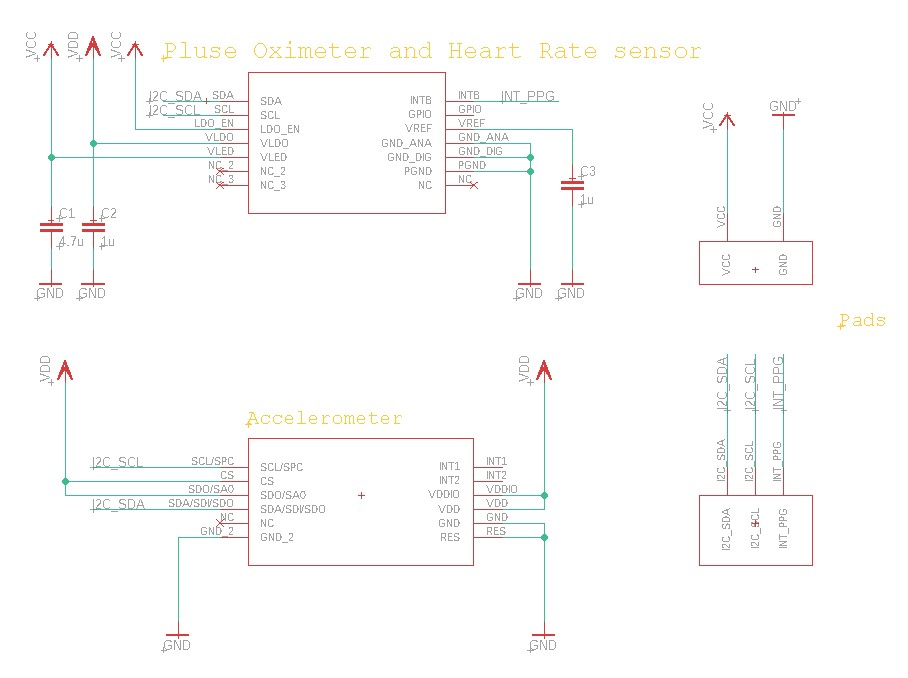
\includegraphics[width=0.8\linewidth]{ImageFiles/Hardware/schematic_maxm}
	\caption{Schematico Adapater Board con il sensore PPG MAXM86161}
	\label{fig:schematic_maxm}
\end{figure}
Il layout è stato progettato partendo dallo schematico, avendo cura di realizzare una board dalle dimensioni più ridotte possibili. Come si può vedere in figura \ref{fig:Layout_maxm} la board si compone su due layer, Top (in rosso) e Bottom (in blu).
\begin{figure}[b]
	\centering
	a$)$
	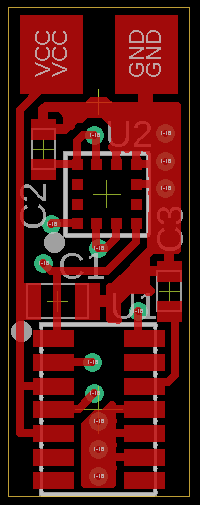
\includegraphics[width=0.1567\linewidth]{ImageFiles/Hardware/layout_top_maxm}
	b$)$
	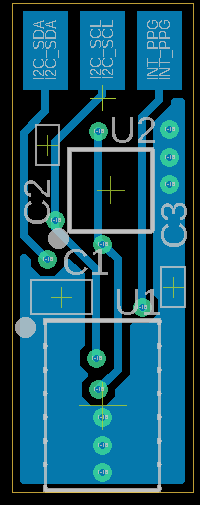
\includegraphics[width=0.1567\linewidth]{ImageFiles/Hardware/layout_bottom_maxm}
	c$)$
	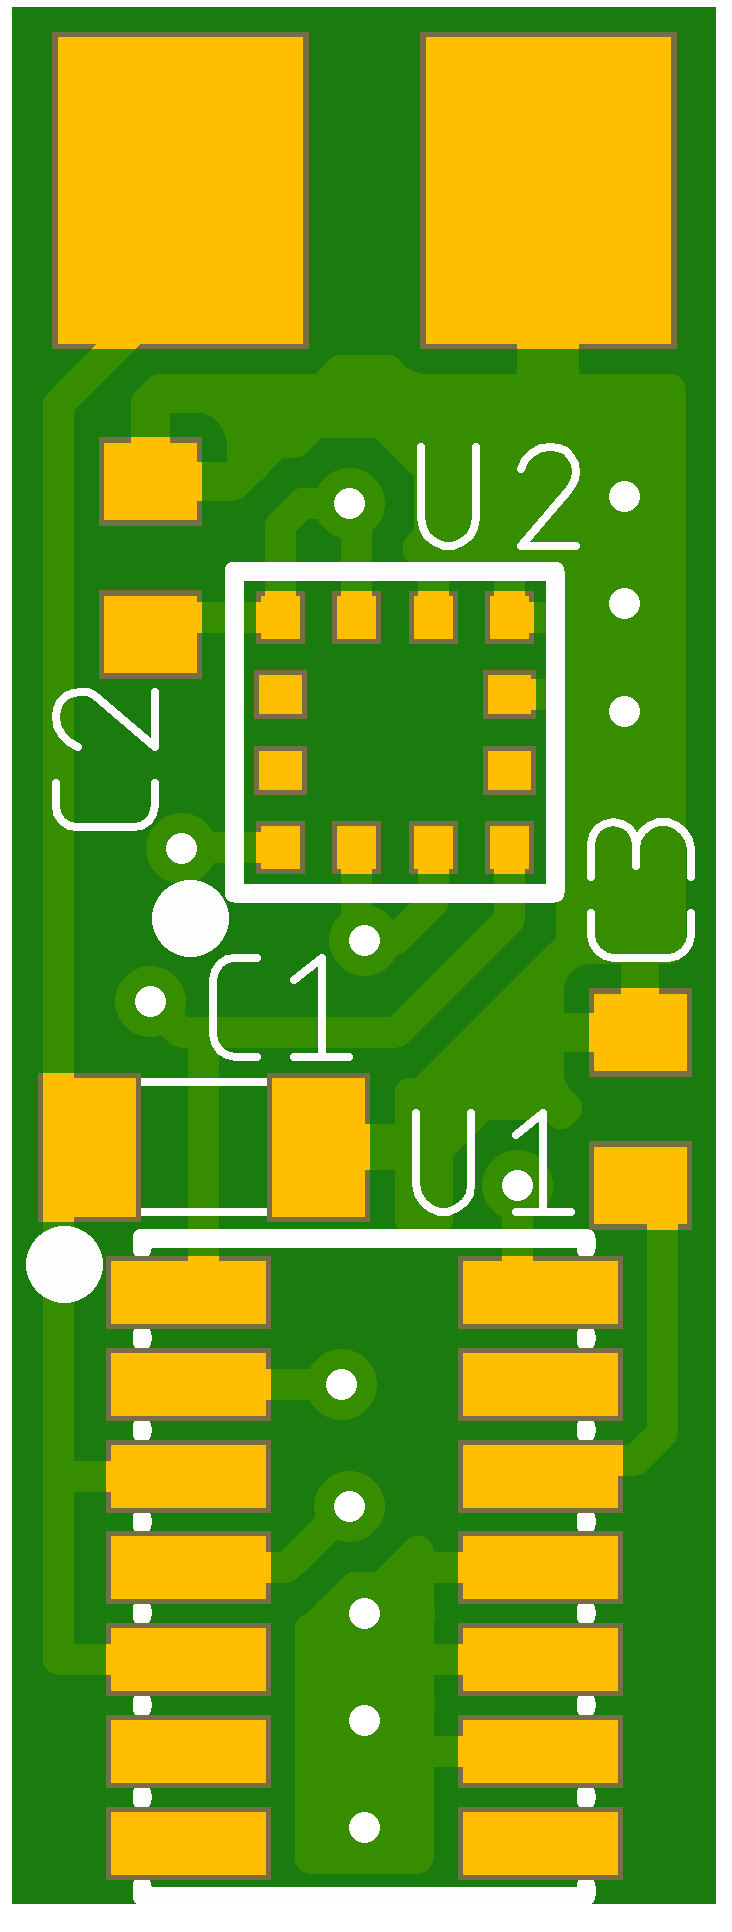
\includegraphics[width=0.15\linewidth]{ImageFiles/Hardware/manifacturing_top_maxm}
	d$)$
	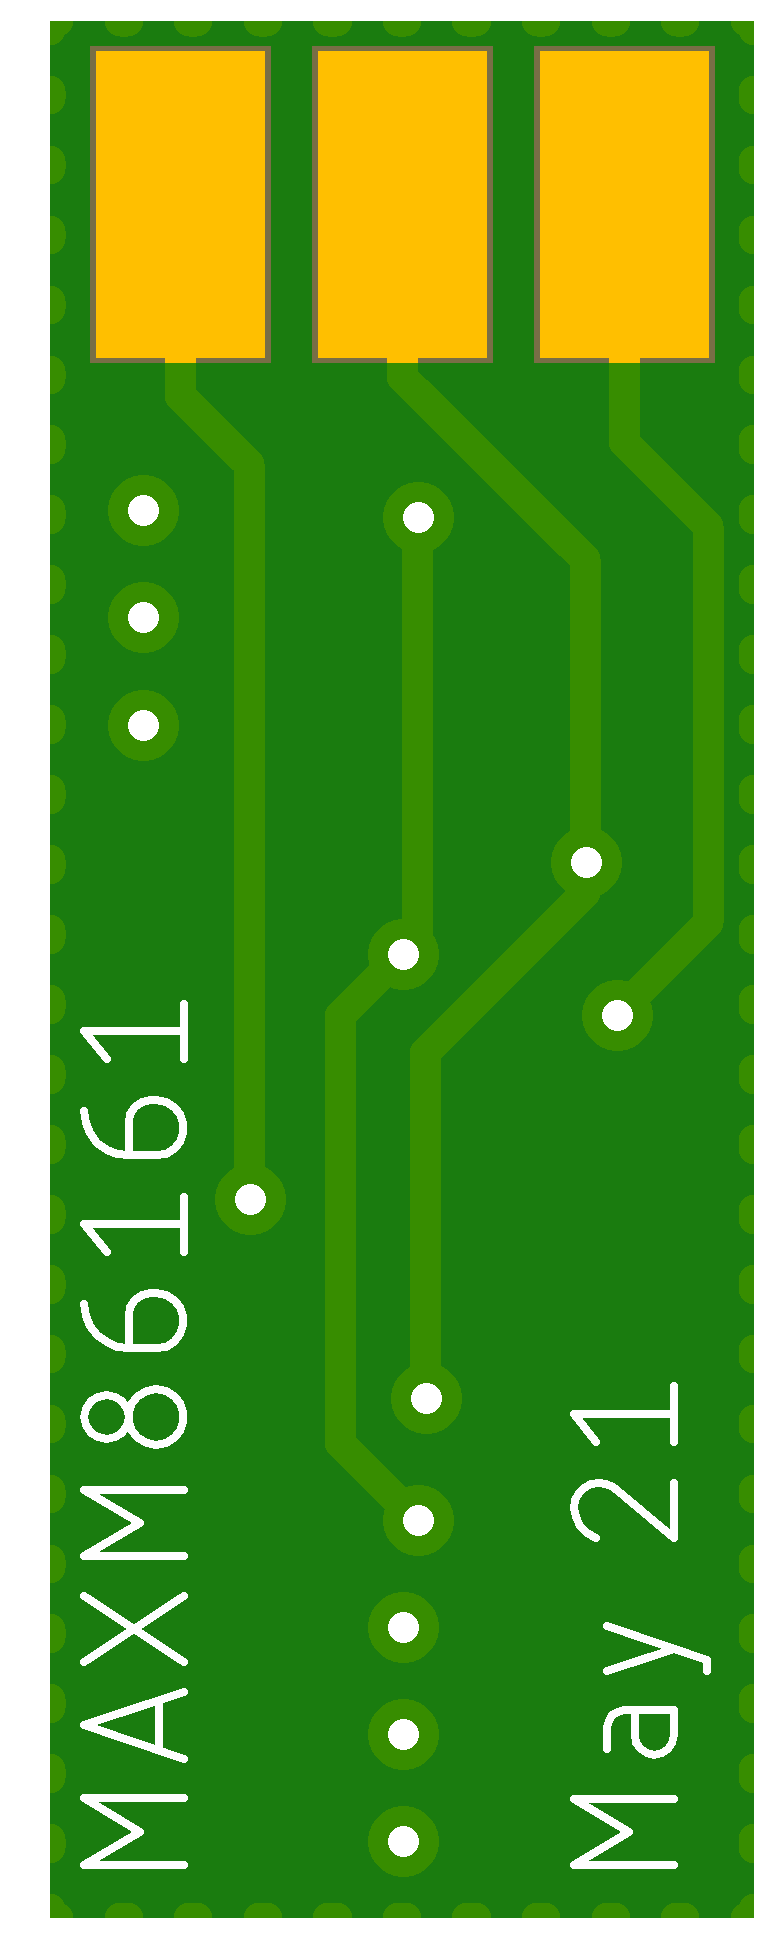
\includegraphics[width=0.15\linewidth]{ImageFiles/Hardware/manifacturing_bottom_maxm}
	\caption{Layout Adapter Board con modulo MAXM86161: a$)$ Livello Top, b$)$ Livello Bottom, c$)$ Rendering 2D Top, d$)$ Rendering 2D Bottom}
	\label{fig:Layout_maxm}
\end{figure}
Le piste disegnate hanno una larghezza di 0.2 mm e dei vias con diametro di 0.2, con una corona di \SI{254}{\micro\meter}.

\pagebreak
Nella tabella \ref{tab:ComponentiAdapterMaxm} vengono riassunti i componenti presenti nell'\textit{Adapter Board} descritta.
\begin{table}[h]
	\renewcommand{\arraystretch}{1.5}
	\centering
	\begin{tabular}{ccccc}
		\hline Nome    & Tipologia   & Principali caratteristiche   \\ 
		\hline MAXM86161 & Sensore PPG  & \begin{tabular}{@{}c@{}}								
			Dimensioni: 2.9mm x 4.3mm x 1.4mm \\ 
			\hline Package: 14 pin - OLGA \\
			\hline Corrente di shutdown: \SI{1.6}{\micro\ampere} \\
			\hline Tensione di alimentazione: 3.0 - 5.5 V \\
			\hline Tensione di uscita LDO: 1.68 - 1.92 V \\
			\hline Protocollo di comunicazione: I\ap{2}C \\
			\hline LED: Rosso, Infrarosso, Verde
		\end{tabular} \\
		\hline LIS2DW12  & Accelerometro triassiale & 
		\begin{tabular}{@{}c@{}}								
			Dimensioni: 2mm x 2mm x 0.7mm \\ 
			\hline Package: LGA-12 \\
			\hline Consumo di shutdown: \SI{50}{\nano\ampere} \\
			\hline Consumo di corrente: \SI{90}{\micro\ampere} \\
			\hline Tensione di alimentazione: 1.62 - 3.6 V \\
			\hline Fondo scala selezionabile: ±2g | ±4g | ±8g | ±16g \\
			\hline Protocollo di comunicazione: I\ap{2}C \\
			\hline Interrupt programmabili: 2 \\
			\hline Orientamento 6D/4D. 
		\end{tabular} \\ 
		\hline
	\end{tabular}
	\caption{Riepilogo dei componenti dell'Adapter Board con sensore MAXM86161.}
	\label{tab:ComponentiAdapterMaxm}
\end{table}
\todo{Cosa da aggiungere?}

\pagebreak
\subsection{Adapter Board: MAX86916}
La seconda Adapter Board progettata è costituita da un modulo PPG MAX86916, da un accelerometro LIS2DW12 e da un LDO (Low-dropout regulator) prodotto da Analog Devices. Come nella board descritta precedentemente, il sensore MAX86916 e l'accelerometro comunicano con il controllore grazie a un'interfaccia standard I\ap{2}C (\Fig~\ref{fig:DiagrammaBlocchiMAX86916}). I dati vengono poi acquisiti da un computer collegato tramite USB alla board STM32F4DISCOVERY, che ospita il microcontrollore. L'aggiunta del regolatore LDO esterno e le dimensioni maggiori del modulo PPG ha portato ad ottenere una PCB con dimensioni 4.5 mm x 17.5 mm. Sebbene siano leggermente maggiori rispetto all'Adapter Board sopra descritta, essa risulta essere molto compatta e adatta ad dispositivi indossabili, con una superficie di solo \SI{78.75}{\square\milli\meter}.
\begin{figure}[h]
	\centering
	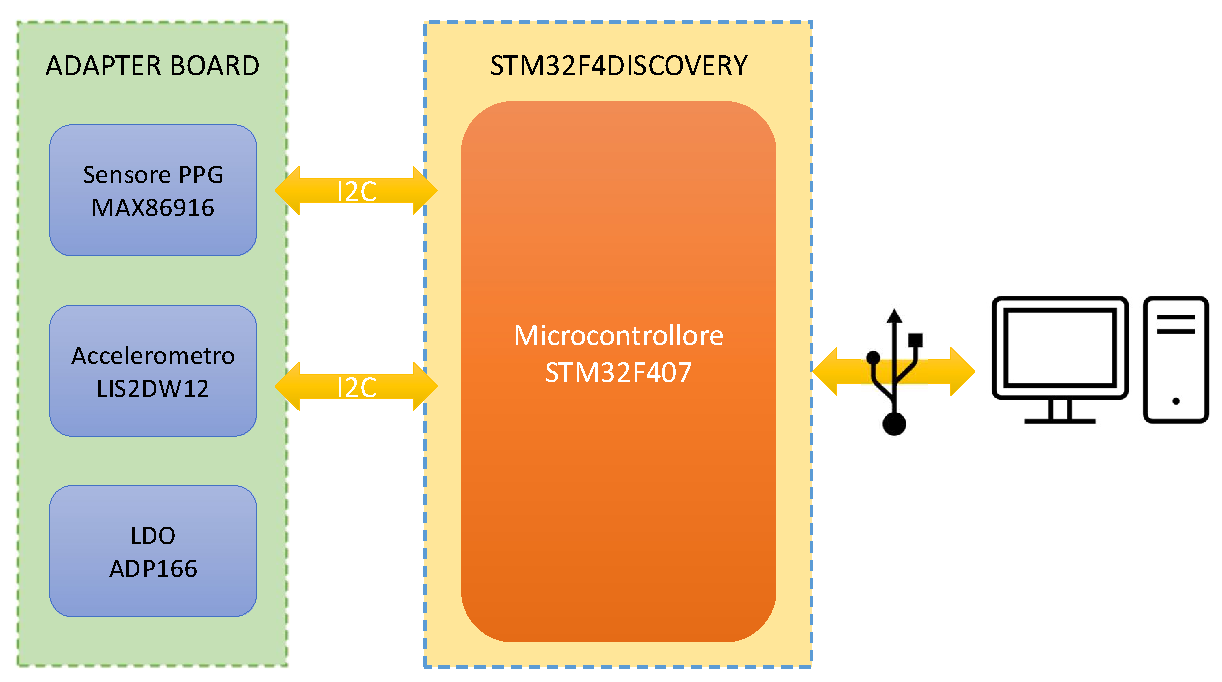
\includegraphics[width=0.6\linewidth]{ImageFiles/Hardware/DiagrammaBlocchiMAX86916}
	\caption{MAX86916 magari mettere in evidenza led e foto diodo}
	\label{fig:DiagrammaBlocchiMAX86916}
\end{figure}

\paragraph{Sensore PPG} Il sensore PPG utilizzato è il \textbf{MAX86916}, prodotto da Maxim Integrated e rappresentato nella figura\ref{fig:ImmagineMAX86916}.
\begin{figure}[b]
	\centering
	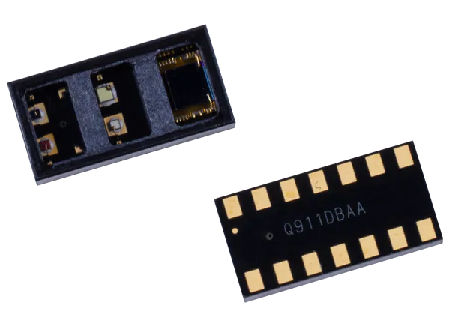
\includegraphics[width=0.6\linewidth]{ImageFiles/Hardware/ImmagineMAX86916}
	\caption{MAX86916 magari mettere in evidenza led e foto diodo}
	\label{fig:ImmagineMAX86916}
\end{figure}
Esso permette l'acquisizione di segnali fotopletismografici grazie a quattro LED, rispettivamente di colore rosso, infrarosso, verde e blu e di un fotodiodo. La peculiarità di questo modulo consiste nella presenza del LED blu, che tipicamente viene omesso. Nel corso di questa tesi, cercheremo di analizzare le caratteristiche delle acquisizioni effettuate con questa lunghezza d'onda (circa \SI{460}{\nano\meter}). Infatti, solitamente vengono utilizzate sorgenti luminose nelle regioni del verde, rosso e infrarosso considerate più efficienti per misure di SpO\ped{2} e HR. I LED vengono alimentati con una tensione di 5.0V \todo{da verificare} fornita dalla scheda STM32F4DISCOVERY, mentre i circuiti interni vengono alimentati con una tensione di 1.8V, grazie al regolatore lineare di tensione. Il modulo si presenta con un package di tipo OLGA a 14 pin con dimensioni 3.5 mm x 7.0 mm x 1.5 mm. Presenta consumi molto ridotti, con una corrente di \SI{0.7}{\micro\ampere} in modalità \textit{shutdown}.

\paragraph{LDO} Per fornire l'alimentazione di al modulo PPG è stato inserito un regolatore lineare di tensione. Il regolatore \textit{low-dropout} è un dispositivo elettronico integrato in grado di fornire una tensione in uscita costante, quando al suo ingresso è applicata un'opportuna tensione\cite{Horowitz2015}.\todo{cit da controllare} In questa Adapter Board, il regolatore viene alimentato con una tensione di 5.0V\todo{da verificare} e fornisce in uscita una tensione di 1.8V che alimenta sia il sensore PPG sia l'accelerometro. Inoltre, sull'ingresso e sull'uscita del LDO sono presenti due condensatori 0402 da \SI{4.7}{\micro\farad} per filtrare eventuali disturbi sulle alimentazioni.

Per la scelta del regolatore da utilizzare in questa Adapter Board, sono stati confrontati diversi LDO disponibili sul mercato e prodotti da Analog Devices: \textbf{ADP166}\cite{AnalogDevicesADP166}, \textbf{ADP122}\cite{AnalogDevicesADP122} e \textbf{ADP151}\cite{AnalogDevicesADP151}. Le loro caratteristiche sono riportarte nella tabella \ref{tab:ConfrontoLDPO}
\begin{table}[h]
	\renewcommand{\arraystretch}{1.5}
	\begin{tabular}{cccc}
		\hline
		& \textbf{ADP166} & \textbf{ADP122} & \textbf{ADP151} \\ \hline
		\textbf{Dimensioni {[}mm\ap{2}{]}}                   & 2 x 2           & 2 x 2           & 2 x 2           \\ \hline
		\textbf{Intervallo tensione in ingresso {[}V{]}}  & 2.2 - 5.5       & 2.3 - 5.5       & 2.2 - 5.5       \\ \hline
		\textbf{Intervallo tensione in uscita {[}V{]}}    & 1.0 - 4.2       & 0.8 - 5         & 1.1 - 3.3       \\ \hline
		\textbf{Tensione di dropout {[}mV{]}}            & 120             & 85              & 140             \\ \hline
		\textbf{Rumore in uscita {[}$\mu$Vrms{]}}         & 80              & 65              & 9               \\ \hline
		\textbf{I\ped{q} Corrente di quiesceza {[}$\mu$A{]}}    & 0.89            & 45              & 10              \\ \hline
		\textbf{I\ped{s} Corrente di shutdown {[}nA{]}}      & 50              & 100             & 200             \\ \hline
		\textbf{I\ped{MAX} Massima corrente erogabile {[}mA{]}} & 150             & 300             & 200             \\ \hline
	\end{tabular}
	\caption{Confronto delle caratteristiche di diversi LDO.}
	\label{tab:ConfrontoLDPO}
\end{table}

\noindent Il modello scelto è l'ADP166, nella versione con tensione fissa di uscita pari a 1.8V e con un package LFCSP di dimesioni 2 mm x 2 mm. La peculiarità di questo LDO risiede nella bassa corrente di quiescenza, pari a circa \SI{890}{\nano\ampere} con un carico da \SI{1}{\micro\ampere}\cite{AnalogDevicesADP166}. Infatti, la \textit{corrente di quiescenza} è definita come la differenza tra la corrente di ingresso e la corrente di uscita\cite{Lee1999}. In altre parole, essa rappresenta la corrente assorbita dal regolatore di tensione e non trasferita al carico. Per questo motivo, dal momento che si vuole progettare una piattaforma indossabile a bassi consumi, avere una bassa corrente di quiescenza significa diminuire i consumi della Adapter Board. Inoltre, l'integrato presenta una bassa corrente di shutdown, che permette di ridurre i consumi quando esso viene disabilitato attraverso il pin EN. Tuttavia, nella nostra piattaforma abbiamo scelto di mantenere il regolatore sempre attivo.

\paragraph{Accelerometro} L'accelerometro utilizzato è il \textbf{LIS2DH12} prodotto da STMicroelectronics, come nell'Adapter Board precedente.

\paragraph{Progetto PCB} Anche il progetto di questa board è stato realizzato con il software Autodesk Eagle. In figura \ref{fig:schematic_max} viene riportato lo schematico dove si possono vedere il sensore PPG, il regolatore di tensione lineare (LDO), l'accelerometro e i connettori per l'alimentazione della scheda e la comunicazione I\ap{2}C.
\begin{figure}[b]
	\centering
	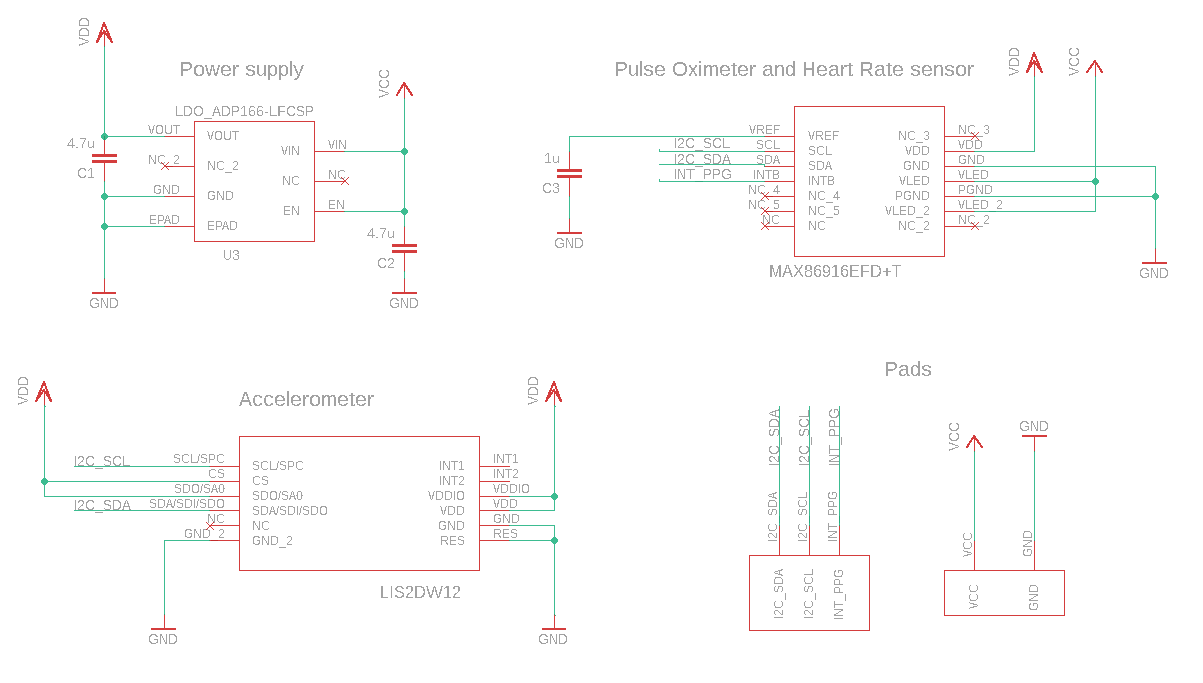
\includegraphics[width=0.8\linewidth]{ImageFiles/Hardware/schematic_max}
	\caption{Schematico Adapater Board con il sensore PPG MAXM86161}
	\label{fig:schematic_max}
\end{figure}
La realizzazione del layout è stata fatta sempre avendo cura di avere una scheda dalle dimensioni ridotte. In figura \ref{fig:Layout_maxm} è riportato il layout della board, che si compone su due layer, Top (in rosso) e Bottom (in blu).
\begin{figure}[tb]
	\centering
	a$)$
	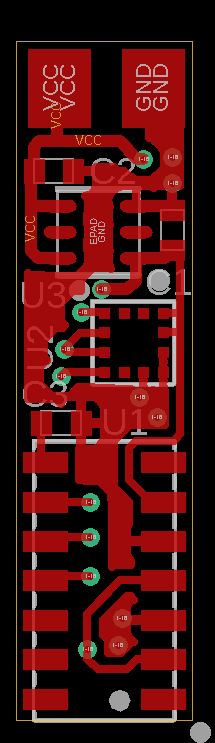
\includegraphics[width=0.1459\linewidth]{ImageFiles/Hardware/layout_top_max}
	b$)$
	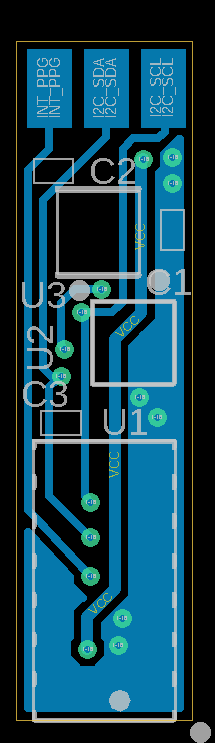
\includegraphics[width=0.1459\linewidth]{ImageFiles/Hardware/layout_bottom_max}
	c$)$
	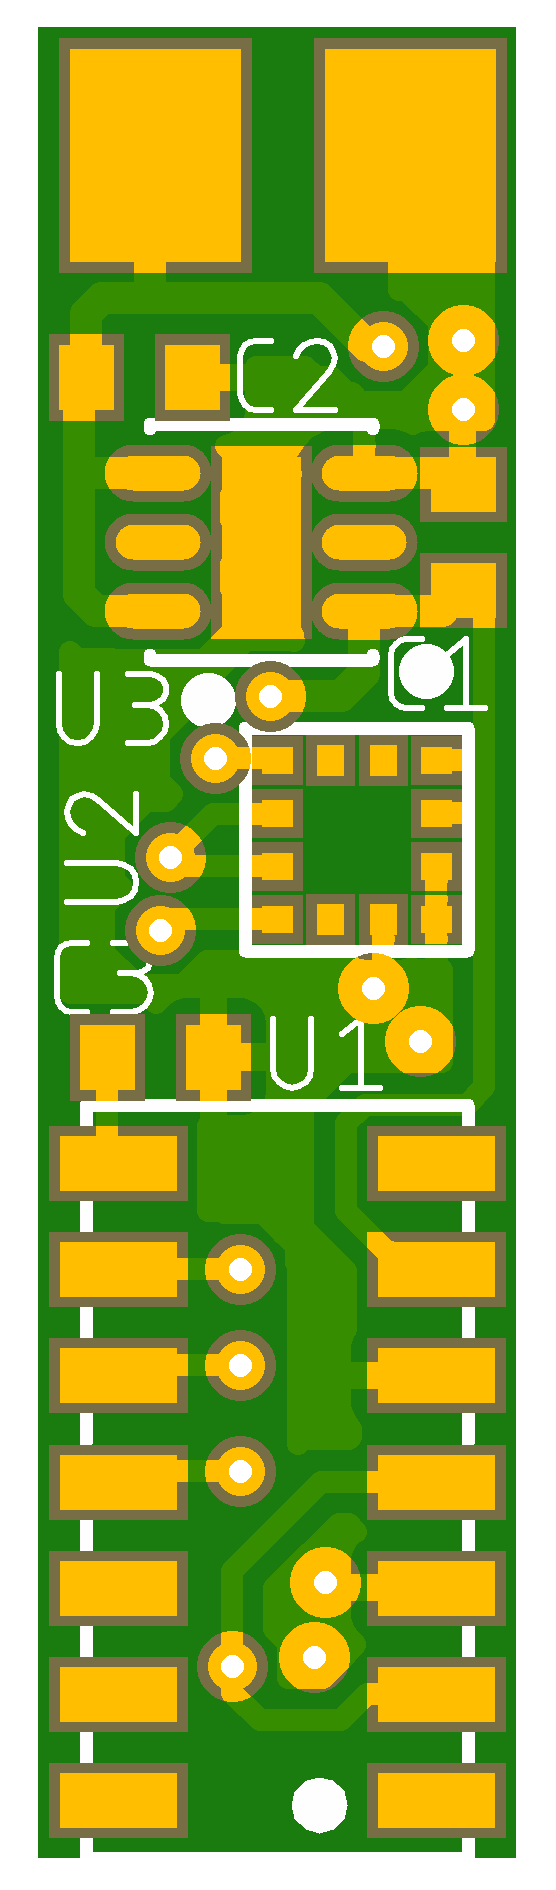
\includegraphics[width=0.16\linewidth]{ImageFiles/Hardware/manifacturing_top_max}
	d$)$
	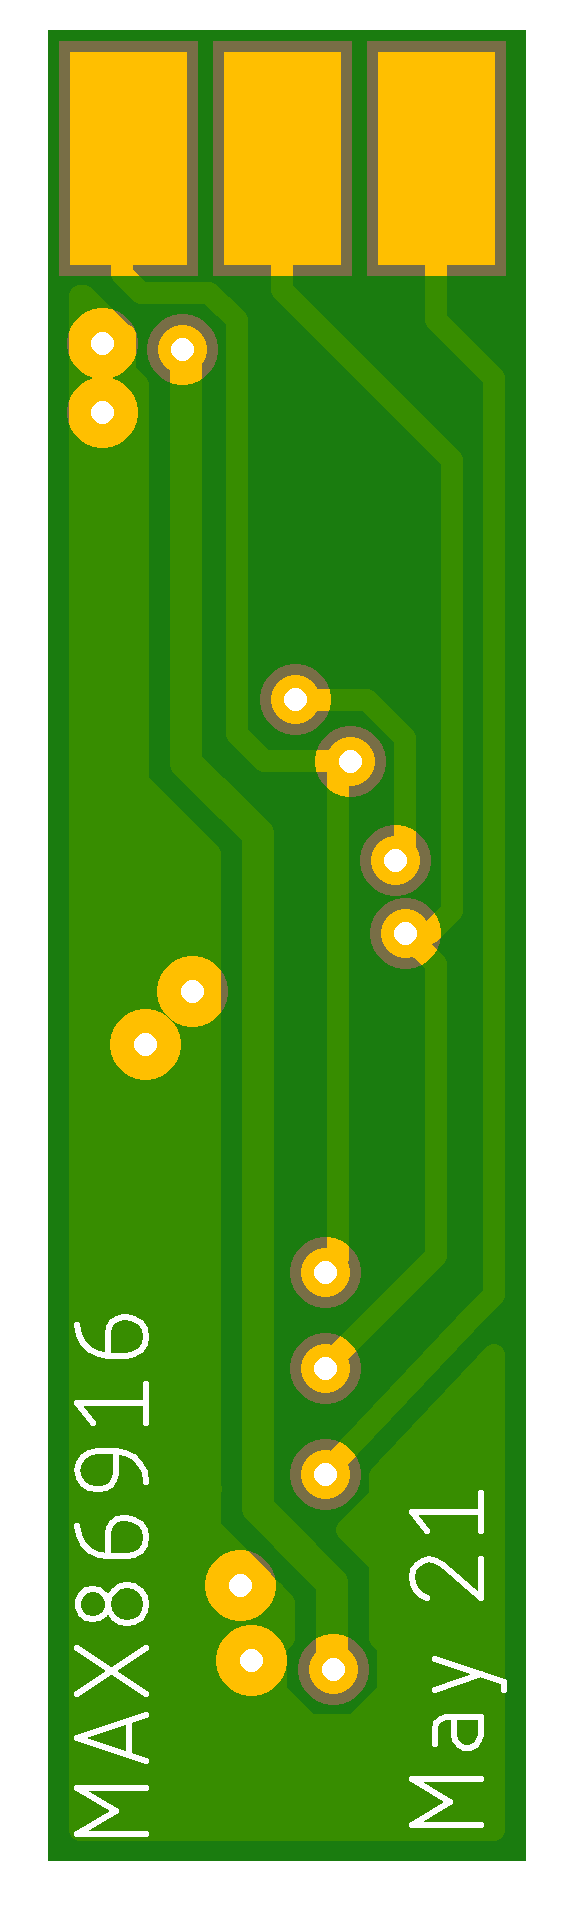
\includegraphics[width=0.16\linewidth]{ImageFiles/Hardware/manifacturing_bottom_max}
	\caption{Layout Adapter Board con modulo MAX86916: a$)$ Livello Top, b$)$ Livello Bottom, c$)$ Rendering 2D Top, d$)$ Rendering 2D Bottom}
	\label{fig:Layout_max}
\end{figure}

\noindent Le piste disegnate hanno una larghezza di 0.2 mm e dei vias con diametro di 0.2, con una corona di \SI{254}{\micro\meter}.
\pagebreak

\noindent Nella tabella \ref{tab:ComponentiAdapterMax} vengono riassunti i componenti presenti nell'\textit{Adapter Board} descritta.
\begin{table}[h]
	\renewcommand{\arraystretch}{1.5}
	\centering
	\begin{tabular}{ccccc}
		\hline Nome    & Tipologia   & Principali caratteristiche   \\ 
		\hline MAX86916 & Sensore PPG  & \begin{tabular}{@{}c@{}}								
			Dimensioni: 3.5mm x 7.0mm x 1.5mm, \\ 
			\hline Package: 14 pin - OLGA \\
			\hline Corrente di shutdown: \SI{0.7}{\micro\ampere} \\
			\hline Tensione di alimentazione PPG: 1.7 - 2.0 V \\
			\hline Tensione di alimentazione LED: 3.5 - 5.5 V \\
			\hline Protocollo di comunicazione: I\ap{2}C \\
			\hline LED: Rosso, Infrarosso, Verde, Blu
		\end{tabular} \\
		\hline ADP166  & Regolatore di tensione lineare (LDO) & \begin{tabular}{@{}c@{}}								
			Dimensioni: 2.0mm x 2.0mm x 1.5mm, \\ 
			\hline Package: 6-lead LFCSP \\
			\hline Corrente di quiescenza: \SI{590}{\nano\ampere} - \SI{890}{\nano\ampere} \\
			\hline Corrente di shutdown: \SI{50}{\nano\ampere} \\
			\hline Massima corrente operativa: \SI{150}{\milli\ampere} \\
			\hline Tensione di ingresso: 2.2 - 5.5 V \\
			\hline Tensione di dropout: \SI{120}{\milli\volt} \\
			\hline Rumore in uscita: \textcolor{red}{\SI{100}{\micro\volt}rms} \\ 
		\end{tabular} \\
		\hline LIS2DW12  & Accelerometro triassiale & vedi sopra \\
	\end{tabular}
	\caption{Riepilogo dei componenti dell'Adapter Board con sensore MAX86916.}
	\label{tab:ComponentiAdapterMax}
\end{table}
\todo{da verificare il rumore e aggiungere l'accelerometro e non vedi sopra}

\pagebreak
\subsection{Microcontrollore: STM32F4DISCOVERY}\todo{farei una descrizione con alcune nozione sui componenti}
\todo{inserire immagine della board}


\todo{alla fine: evidenziare in grassetto la prima volta che compaiono i componenti nei paragrafi componenti}

\clearpage